Let $f(A)$ be a function over a $n\times 1$ vector $A$ such that $f$ can be computed by a $L-$uniform arithmetic circuit of log-depth. Each gate of the circuit that encodes $f$ has an $\texttt{id}\in\lbrace 0,1 \rbrace^n$. From now on, when we write $g$ for a gate of the circuit, we mean the $\texttt{id}$ encoding $g$.
Let $n^k$ be a polynomial such that the number of wires $W(n)\leq n^k$ for $n$ big enough. Further, we assume that $2W(n)\leq n^k$. We need this because the for-matlang simulation of the circuit is in a depth first search way, so $2W(n)$ wires will be traversed.
Then we have that:
\begin{itemize}
	\item the number of gates is bounded by $n^k$.
	\item we need at most $k\log (n)$ bits to store the $id$ of a gate.
	\item the depth of the circuit is at most $k'\log (n)$ for some $k'$.
\end{itemize}

So, let $n_0$ and $k$ such that $\forall n\geq n_0:$

\begin{align*}[right=\empheqrbrace (\star)]
    2W(n)&\leq n^k \\
	k \ceil{\log (n)} &\leq n-3 \\
	k' \ceil{\log(n)} &\leq n
\end{align*}

We know $n_0$ and $k$ exist. Let $n\geq n_0$. Towards the end, we will deal with the case when $n<n_0$.

Let $g$ be a gate. The children of $g$ are denoted by $g_1,\ldots, g_l$.
\begin{center}
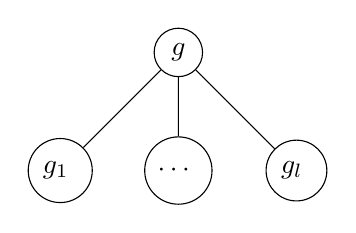
\begin{tikzpicture}[level distance=1.5cm,
  level 1/.style={sibling distance=1.5cm},
  every node/.style = {
  	shape=circle,
    draw,
    align=center,
    top color=white,
    bottom color=white
    }]
  \node {\( g \)}
    child {node { \( g_1 \) }}
    child {node { \( \cdots \) }}
    child {node { \( g_l \) }};
\end{tikzpicture}
\end{center}

For example, a circuit that encodes the function $f(a_1,a_2,a_3,a_4)=a_1a_2 +a_3a_4$ is 

\begin{center}
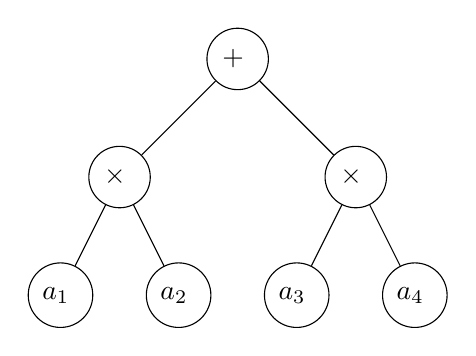
\begin{tikzpicture}[level distance=1.5cm,
  level 1/.style={sibling distance=3cm},
  level 2/.style={sibling distance=1.5cm},
  every node/.style = {
  	shape=circle,
    draw,
    align=center,
    top color=white,
    bottom color=white
    }
  ]
  \node { \( + \) }
    child { node { \( \times \) }
      child { node { \( a_1 \) } }
      child {node { \( a_2 \) } }
    }
    child { node { \( \times \) }
      child { node { \( a_3 \) } }
      child { node { \( a_4 \) } }
    };
\end{tikzpicture}
\end{center}

We can simulate the polynomial $x^2+xy$ by doing $f(A)$ where $A=[x \hspace{1ex} x \hspace{1ex} x \hspace{1ex} y]^*$. The main idea is to traverse the circuit top down in a depth first search way and store visited gates in a stack and its corresponding current values in another stack, and aggregate in the iterations according to the gate type.

For a stack $S$, the operations are standard:

\begin{itemize}
	\item $\push{S}{s}$: pushes $s$ into $S$.
	\item $\pop{S}$: pops the top element.
	\item $\getsize{S}$: the length of the stack.
	\item $\gettop{S}$: the top element in the stack.
\end{itemize}

For the pseudo-code, $\cG$ and $\cV$ denote stacks of gates and values, respectively. The property that holds during the simulation is that the value in $\cV[i]$ is the value that $\cG[i]$ currently outputs. The algorithm ends with $\cG=\left[ g_{\texttt{root}}\right]$ and $\cV=\left[ v_{\texttt{root}}\right]$ after traversing the circuit, and returns $v_{\texttt{root}}$

During the evaluation algorithm there will be two possible configurations of $\cG$ and $\cV$.

\begin{enumerate}
	\item $\getsize{\cG} = \getsize{\cV} + 1$: this means that $\gettop{\cG}$ is a gate that we visit for the first time and we need to initialize its value.
	
	\item $\getsize{\cG} = \getsize{\cV}$: here $\gettop{\cV}$ is the value of evaluating the circuit in gate $\gettop{\cG}$. Therefore, we need to aggregate the value $\gettop{\cV}$ to the parent gate of $g$.
\end{enumerate}

We assume the circuit has input gates, $+, \times$-gates and allow constant $1$-gate.

The idea is to traverse the circuit top down in a depth first search way. For example, in the circuit $f(a_1,a_2,a_3,a_4)=a_1a_2 +a_3a_4$ above, we would initialize the output gate value as $0$ because it is a $+$ gate, so $\cG=\lbrace +\rbrace$, $\cV=\lbrace 0\rbrace$. Then stack the left $\times$ gate to $\cG$, stack its initial value (i.e. $1$) to $\cV$. Now stack $a_1$ to $\cG$ and its value (i.e. $a_1$) to $\cV$. Since we are on an input gate we pop the gate and value pair off of $\cG$ and $\cV$ respectively, aggregate $a_1$ to $\gettop{\cV}$ and continue by stacking the $a_2$ gate to $\cG$. We pop $a_2$ off of $\cV$ (and its gate off of $\cG$) and aggregate its value to $\gettop{\cV}$. We pop and aggregate the value of the left $\times$ gate to $\gettop{\cV}$ (the root value). Then continue with the right $\times$ gate branch similarly.

For the pseudo-code, we supply ourselves with the following functions:

\begin{itemize}
	\item[--] $\isplus{g}$: true if and only if $g$ is a $+$-gate.
	\item[--] $\isprod{g}$: true if and only if $g$ is a $\times$-gate.
	\item[--] $\isone{g}$: true if and only if $g$ is a $1$-gate.
	\item[--] $\isinput{g}$: true if and only if $g$ is an input gate.
	\item[--] $\getfirst{g}$: outputs the first child of $g$.
	\item[--] $\getinput{g}$: outputs $A[i]$ when $g$ is the $i$-th input.
	\item[--] $\isnotlast{g_1}{g_2}$: true if and only if $g_2$ is not the last child gate of $g_1$.
	\item[--] $\nextgate{g_1}{g_2}$: outputs the next child gate of $g_1$ after $g_2$.
	\item[--] $\getroot$: outputs the root gate of the circuit.
\end{itemize}

The corresponding $\lbrace 0,1 \rbrace^n\rightarrow\lbrace 0,1 \rbrace^n$ functions are:

\begin{itemize}
	\item[--] $\isplus{g}$: $1$ if and only if $g$ is a $+$-gate.
	\item[--] $\isprod{g}$: $1$ if and only if $g$ is a $\times$-gate.
	\item[--] $\isone{g}$: $1$ if and only if $g$ is a $1$-gate.
	\item[--] $\isinput{g}$: $1$ if and only if $g$ is an input gate.
	\item[--] $\getfirst{g}$: outputs the $\texttt{id}$ of the first child of $g$.
	\item[--] $\getinput{g}$: outputs $e_i$ where the $i$-th input gate of $A$ is encoded by $g$.
	\item[--] $\isnotlast{g_1}{g_2}$: $1$ if and only if $g_2$ is not the last child gate of $g_1$.
	\item[--] $\nextgate{g_1}{g_2}$: outputs the $\texttt{id}$ of the next child gate of $g_1$ after $g_2$.
	\item[--] $\getroot$: outputs the $\texttt{id}$ of the root gate of the circuit.
\end{itemize}

The previous functions are all definable by an $L$-transducer and can be defined from the $L$-transducer of $f$. Then, for each of these functions, there is a \langfor expression that simulates them.

Now, we give the pseudo-code of the top-down evaluation. We define the functions $Initialize$ (algorithm \ref{alg:init_code}), $Aggregate$ (algorithm \ref{alg:agg_code}) and $Evaluate$ (algorithm \ref{alg:eval_code}). The main algorithm is $Evaluate$.

\begin{algorithm}
\caption{Initialize (pseudo-code)}\label{alg:init_code}
\begin{algorithmic}[1]
\Function{Initialize}{$\cG, \cV, A$}\Comment{The stacks and input. Here, $\getsize{\cG} =  \getsize{\cV} + 1$}
	\If{$\isplus{\gettop{\cG}}$}
		\State $\push{\cV}{0}$
		\State $\push{\cG}{\getfirst{\gettop{\cG}}}$
	\ElsIf{$\isprod{\gettop{\cG}}$}
		\State $\push{\cV}{1}$
		\State $\push{\cG}{\getfirst{\gettop{\cG}}}$
	\ElsIf{$\isone{\gettop{\cG}}$}
		\State $\push{\cV}{1}$
	\ElsIf{$\isinput{\gettop{\cG}}$}
		\State $\push{\cV}{A\left[ \getinput{\gettop{\cG}} \right]}$
	\EndIf
	\State \textbf{return} $\cG, \cV$
\EndFunction
\end{algorithmic}
\end{algorithm}

\begin{algorithm}
\caption{Aggregate (pseudo-code)}\label{alg:agg_code}
\begin{algorithmic}[1]
\Function{Aggregate}{$\cG, \cV$}\Comment{Here, $\getsize{\cG} =  \getsize{\cV}$}
	\State $g = \pop{\cG}$
	\State $v = \pop{\cV}$
	\If{$\isplus{\gettop{\cG}}$}
		\State $\gettop{\cV} = \gettop{\cV} + v$
	\ElsIf{$\isprod{\gettop{\cG}}$}
		\State $\gettop{\cV} = \gettop{\cV} \cdot v$
	\EndIf
	\If{$\isnotlast{\gettop{\cG}}{g}$}
		\State $\push{\cG}{\nextgate{\gettop{\cG}}{g}}$
	\EndIf
	\State \textbf{return} $\cG, \cV$
\EndFunction
\end{algorithmic}
\end{algorithm}

\begin{algorithm}
\caption{Evaluate (pseudo-code)}\label{alg:eval_code}
\begin{algorithmic}[1]
\Function{Evaluate}{$A$}\Comment{Input $ n\times 1$ vector $A$. Here, $\cG$ and $\cV$ are empty}
	\State $\push{\cG}{\getroot}$
	\While{$\getsize{\cG}\neq 1$ or $\getsize{\cV}\neq 1$}
		\If{$\getsize{\cG}\neq \getsize{V}$}
			\State $(\cG,\cV) := \texttt{Initialize}(\cG,\cV,A)$
		\Else
			\State $(\cG,\cV):= \texttt{Aggregate}(\cG,\cV)$
		\EndIf
	\EndWhile
	\State \textbf{return} $\gettop{\cV}$
\EndFunction
\end{algorithmic}
\end{algorithm}

The $Evaluate$ algorithm gives us the output of the circuit. Note that after each iteration it either holds that $\getsize{\cG} =  \getsize{\cV} + 1$ or $\getsize{\cG} =  \getsize{\cV}$. Furthermore, when we start we have $\getsize{\cG}=1$ and $\getsize{\cV}=0$. The condition $\getsize{\cG}= 1$ and $\getsize{\cV}=1$ holds only when we have traversed all the circuit, and the value in $\gettop{\cV}$ is the value that the root of the circuit outputs after its computation.

Next, we show how to encode this algorithm in $\langfor$.

Let $n_0\in\mathbb{N}$ be big enough for $\star$ to hold and let $n\geq k$. Hence, the number of gates (values) is bounded by $n^k$ and we need $k\log (n)$ bits to encode the id of each gate.

To simulate the two stacks $\cG$ and $\cV$ we keep a matrix $X$ of dimensions $n \times n$.

\begin{itemize}
	\item Column $n$ will store a canonical vector that marks the top of stack $V$ (values).
	\item Column $n-1$ will store a canonical vector that marks the top of stack $G$ (gates).
	\item Column $n-2$ is the stack of values where $X[1, n-2]$ is the bottom of the stack.
	\item Columns $1$ to $n-3$ are the stack of gates.
\end{itemize}

If we have $j$ gates in the stack and currently $\getsize{\cG}=\getsize{\cV}$ then $X$ would look like:

\[
X = \begin{bmatrix}
    \texttt{id}_1 & v_1 & 0 & 0 \\
    \texttt{id}_2 & v_2 & 0 & 0 \\
    \vdots & \vdots & \vdots & \vdots \\
    \texttt{id}_j & v_j & 1 & 1 \\
    0 & 0 & 0 & 0 \\
    \vdots & \vdots & \vdots & \vdots \\
     0 & 0 & 0 & 0
\end{bmatrix}.
\]

Since $n\geq n_0$, $(\star)$ holds and thus we never use more than $n-3$ bits to encode an $\texttt{id}$. Also, $j\leq n$ given that we never keep more gates than the depth of the tree. As a consequence, we never keep more than $n$ values either.

\thomas{The following remark is necessary because of dimensions (check typing of START). I don't know if the reverse part is correct, but it makes sense to me since that way zeroes to the right actually mean nothing in the binary number (if it is reversed).}

An important detail is that the $\texttt{ids}$ of the gates are encoded as $\texttt{id}_r000$ for it to have dimension $n$, where $\texttt{id}_r$ is the corresponding binary number in reverse.

We make a series of definitions to make the notation more clear.

Let $e_i$ be the $i$-th canonical vector. $S$ and $P$ denote the successor and predecessor matrices respectively, such that

\[
  			S\cdot e_i=\begin{cases}
               e_{i+1} \text{ if } i\leq n \\
               \mathbf{0} \text{ otherwise }
            \end{cases}
\]

\[
  			P\cdot e_i=\begin{cases}
               e_{i-1} \text{ if } i\geq n \\
               \mathbf{0} \text{ otherwise }
            \end{cases}
\]

We write $e_{min}$ for the first canonical vector and $e_{max}$ for the last canonical vector. For any $i$ we write 
\begin{align*}
	e_{min+i} &= S^i\cdot e_{min} \\
	e_{max+i} &= P^i\cdot e_{max}
\end{align*}

We use the extra $\lbrace 0,1 \rbrace^n\rightarrow\lbrace 0,1 \rbrace^n$ functions that have a $\langfor$ translation:

\[
  			min(e)=\begin{cases}
               1 \text{ if } e=e_{min} \\
               0 \text{ otherwise }
             \end{cases}
\]

\[
  			max(e)=\begin{cases}
               1 \text{ if } e=e_{max} \\
               0 \text{ otherwise }
             \end{cases}
\]

\[
  			less(e_i,e_j)=\begin{cases}
               1 \text{ if } i\leq j \\
               0 \text{ otherwise }
             \end{cases}
\]

When used in $\langfor$ these functions output $[0]$ and $[1]$.

Now 
\begin{align*}
	e_{V}&:=e_{max-2} \\
	e_{G_{top}}&:=e_{max-1} \\
	e_{V_{top}}&:=e_{max}
\end{align*}

For a canonical vector, let $$\Iden{e_i}:=\ssum v. less(v,e_i)\cdot (v\cdot v^*).$$ This matrix has ones in the diagonal up to position $i$ marked by $e_{i}$. We define the following sub-matrices of $X$:
\begin{align*}
	V_{top} &:= X\cdot e_{V_{top}} \\
	V &:= \Iden{V_{top}} \cdot X \cdot e_v \\
 	G_{top} &:=X\cdot e_{G_{top}} \\
 	G &:= \Iden{G_{top}}\cdot X \cdot \Iden{e_{max-3}}
\end{align*}

For example, if we are in a step where $\getsize{\cG}=\getsize{\cV} + 1$ then

\[
X = \begin{bmatrix}
    \texttt{id}_1 & v_1 & 0 & 0 \\
    \texttt{id}_2 & v_2 & 0 & 0 \\
    \vdots & \vdots & \vdots & \vdots \\
    \texttt{id}_{j-1} & v_{j-1} & 0 & 1 \\
    \texttt{id}_j & 0 & 1 & 0 \\
    0 & 0 & 0 & 0 \\
    \vdots & \vdots & \vdots & \vdots \\
     0 & 0 & 0 & 0
\end{bmatrix}, 
G = \begin{bmatrix}
    \texttt{id}_1  \\
    \texttt{id}_2 \\
    \vdots   \\
    \texttt{id}_{j-1} \\
    \texttt{id}_j \\
    0 \\
    \vdots \\
     0 
\end{bmatrix}, 
V = \begin{bmatrix}
    v_1  \\
    v_2 \\
    \vdots   \\
    v_{j-1} \\
    0 \\
    0 \\
    \vdots \\
     0 
\end{bmatrix}, 
G_{top} = \begin{bmatrix}
    0  \\
    0 \\
    \vdots   \\
    0 \\
    1 \\
    0 \\
    \vdots \\
     0 
\end{bmatrix}, 
V_{top} = \begin{bmatrix}
    0  \\
    0 \\
    \vdots   \\
    1 \\
    0 \\
    0 \\
    \vdots \\
     0 
\end{bmatrix}
\]

Here, $V$ is a vector encoding the stack of values in $X$ and $G$ is a matrix encoding the stack of gates in $X$. Note that what is \textit{over} the top of the stacks is always set to zero due to $\Iden{G_{top}}$ and $\Iden{V_{top}}$.

To set the initial state (algorithm \ref{alg:eval_code} line 2) we define the $\langfor$ expression: $$\text{START}:= e_{min}\cdot \getroot^* + e_{min}\cdot e_{G_{top}}^*.$$
For the initialize step, we define the $\langfor$ expressions: INIT${\_}$PLUS (algorithm \ref{alg:init_code}, lines 2, 3, 4), INIT${\_}$PROD (algorithm \ref{alg:init_code}, lines 5, 6, 7), CONST (algorithm \ref{alg:init_code}, lines 8, 9) and INPUT (algorithm \ref{alg:init_code}, lines 10, 11):

\begin{align*}
	\text{INIT{\_}PLUS} &:= \isplus{G^*\cdot G_{top}}\odot \left[ G + S\cdot G_{top} \cdot \getfirst{G^*\cdot G_{top}}^*  + S\cdot G_{top}\cdot e_{G_{top}}^* +V\cdot e_{V} + S\cdot V_{top}\cdot e_{V_{top}}^* \right] \\
	\text{INIT{\_}PROD} &:= \isprod{G^*\cdot G_{top}}\odot \left[ G + S\cdot G_{top} \cdot \getfirst{G^*\cdot G_{top}}^* + S\cdot G_{top}\cdot e_{G_{top}}^* +(V + S\cdot v_{top})\cdot e_{V} + S\cdot V_{top}\cdot e_{V_{top}}^* \right] \\
	\text{CONST} &:= \isone{G^*\cdot G_{top}}\odot \left[ G + (V + S\cdot v_{top})\cdot e_{V} + S\cdot V_{top}\cdot e_{V_{top}}^* \right] \\
	\text{INPUT} &:= \isinput{G^*\cdot G_{top}}\odot \left[ G + \left(V + \left( A^* \cdot \getinput{G^*\cdot G_{top}} \cdot S\cdot V_{top} \right)\right)\cdot e_{V} + S\cdot V_{top}\cdot e_{V_{top}}^* \right]
\end{align*} 

Here, $G^*\cdot G_{top}$ is to get the current id in the top of the stack. In INIT${\_}$PLUS we get the current stack $G$, we add $S\cdot G_{top} \cdot \getfirst{G^*\cdot G_{top}}^*$ which is an $n\times n$ matrix with the first child of $G^*\cdot G_{top}$, then $S\cdot G_{top}\cdot e_{G_{top}}^*$ adds $S\cdot G_{top}$ to the $n-1$ column to mark the gate we added as the top. Next, we do the same with the values by adding $V\cdot e_{V} + S\cdot V_{top}\cdot e_{V_{top}}^*$

The $\langfor$ expression equivalent to algorithm \ref{alg:init_code} is $$\text{INIT}:=\text{INIT{\_}PLUS}+\text{INIT{\_}PROD}+\text{CONST}+\text{INPUT}.$$

The idea is to return the matrix for the next iteration. Recall that here $\getsize{\cG}=\getsize{\cV} + 1$. So, when the operation is INPUT or CONST, if we start with

\[
\begin{bmatrix}
    \texttt{id}_1 & v_1 & 0 & 0 \\
    \texttt{id}_2 & v_2 & 0 & 0 \\
    \vdots & \vdots & \vdots & \vdots \\
    \texttt{id}_{j-1} & v_{j-1} & 0 & 1 \\
    \texttt{id}_j & 0 & 1 & 0 \\
    0 & 0 & 0 & 0 \\
    \vdots & \vdots & \vdots & \vdots \\
     0 & 0 & 0 & 0
\end{bmatrix}, \text{ then we return }
\begin{bmatrix}
    \texttt{id}_1 & v_1 & 0 & 0 \\
    \texttt{id}_2 & v_2 & 0 & 0 \\
    \vdots & \vdots & \vdots & \vdots \\
    \texttt{id}_{j-1} & v_{j-1} & 0 & 0 \\
    \texttt{id}_j & v_j & 1 & 1 \\
    0 & 0 & 0 & 0 \\
    \vdots & \vdots & \vdots & \vdots \\
     0 & 0 & 0 & 0
\end{bmatrix}.
\]

When the operation is INIT{\_}PLUS or INIT{\_}PROD, if we start with 

\[
\begin{bmatrix}
    \texttt{id}_1 & v_1 & 0 & 0 \\
    \texttt{id}_2 & v_2 & 0 & 0 \\
    \vdots & \vdots & \vdots & \vdots \\
    \texttt{id}_{j-1} & v_{j-1} & 0 & 1 \\
    \texttt{id}_j & 0 & 1 & 0 \\
    0 & 0 & 0 & 0 \\
    0 & 0 & 0 & 0 \\
    \vdots & \vdots & \vdots & \vdots \\
     0 & 0 & 0 & 0
\end{bmatrix}, \text{ then we return }
\begin{bmatrix}
    \texttt{id}_1 & v_1 & 0 & 0 \\
    \texttt{id}_2 & v_2 & 0 & 0 \\
    \vdots & \vdots & \vdots & \vdots \\
    \texttt{id}_{j-1} & v_{j-1} & 0 & 0 \\
    \texttt{id}_j & v_j & 0 & 1 \\
    \texttt{id}_{j+1} & 0 & 1 & 0 \\
    0 & 0 & 0 & 0 \\
    \vdots & \vdots & \vdots & \vdots \\
     0 & 0 & 0 & 0
\end{bmatrix}.
\]


For the aggregate expression (algorithm \ref{alg:agg_code}) we do the following. Let $$\pondIden{e_i}{c}=\ssum v. (v^*\cdot e_i)\cdot c\cdot v\cdot v^* + (1-v^*\cdot e_i)\cdot v \cdot v^*,$$ namely, it is the identity with $c$ in position $(i,i)$.

We define the expressions: AGG${\_}$PLUS (algorithm \ref{alg:agg_code}, lines 4, 5), AGG${\_}$PROD (algorithm \ref{alg:agg_code}, lines 6, 7),  IS${\_}$NOT${\_}$LAST (algorithm \ref{alg:agg_code}, lines 8, 9), IS${\_}$LAST and POP:

\begin{align*}
	\text{POP} &:= \Iden{P\cdot G_{top}}\cdot G + P\cdot V_{top}\cdot e_{V_{top}}^*  \\
	\text{AGG{\_}PLUS} &:= \isplus{G^* \cdot \left( P \cdot G_{top}\right)} \odot \left[ \left( \Iden{P\cdot V_{top}} \cdot V + \left( V^* \cdot V_{top} \right)\left( P\cdot V_{top} \right)\right) \cdot e_{V}^* \right] \\
	\text{AGG{\_}PROD} &:= \isprod{G^* \cdot \left( P \cdot G_{top}\right)} \odot \left[ \left( \pondIden{P\cdot V_{top}}{V^* \cdot V_{top}} \cdot \Iden{P\cdot V_{top}} \cdot V \right) \cdot e_{V}^* \right] \\
	\text{IS{\_}NOT{\_}LAST} &:= \isnotlast{G^* \cdot \left( P \cdot G_{top}\right)}{G^* \cdot G_{top}} \odot \left[  G_{top} \cdot \nextgate{G^* \cdot \left( P\cdot G_{top} \right) }{G^* \cdot G_{top}} + G_{top}\cdot e_{G_{top}}^* \right] \\
	\text{IS{\_}LAST} &:= \left( 1 - \isnotlast{G^* \cdot \left( P \cdot G_{top}\right)}{G^* \cdot G_{top}} \right)\odot \left[ \left( P\cdot G_{top} \right) \cdot e_{G_{top}}^* \right]
\end{align*}

The $\langfor$ expression equivalent to algorithm \ref{alg:agg_code} is $$\text{AGG}:=\text{POP} + \text{AGG{\_}PLUS}+\text{AGG{\_}PROD}+\text{IS{\_}NOT{\_}LAST}+\text{IS{\_}LAST}.$$

The $Evaluate$ method (algorithm \ref{alg:eval_code}) is defined as follows:

\begin{align*}
	\text{EVAL}&[A]= \\
	&e_{min}^* \cdot \ffor{X}{v_1, \ldots, v_k}: \big\lbrace \\
	&\left( \sprod_{i=1}^k min(v_i)\right) \odot START + \\
	&\left( 1- \sprod_{i=1}^k min(v_i)\right) \odot \left( \left(1 - min(G_{top})\cdot min(V_{top}) \right) \odot \left[ \left( 1 - G_{top}^*\cdot V_{top} \right) \odot \text{INIT} + \left(  G_{top}^*\cdot V_{top} \right) \odot \text{AGG} \right] + min(G_{top})\odot min(V_{top})\odot X\right) \\ 
	&\big\rbrace \cdot e_{V}
\end{align*}

Note that the $ \texttt{for}$-expression does the evaluation. The final output is in $X[1,max-2]$, we extract this value by multiplying the final result as $e_{min}^*\cdot [\texttt{for}(\ldots )]\cdot e_{V}$.

Finally, we need to take care of all $n<n_0$, where $(\star)$ does not necessarily hold. For any $i$, let: $$\text{Eval}[i,A]:= \text{ the } 1\times 1 \text{ matrix with the value of the polynomial } f(A) \text{ when } n=i.$$

Then we define: $$f(A)=\ssum_{i=0}^{n_0-1}(e_{min+i}\cdot e_{max}^*)\odot \text{EVAL}[i,A] + \left( (S^{n_0}\cdot e_{min})^*\cdot \ones (e_{min}) \right)\odot \text{EVAL}[A].$$ Above, $(e_{min+i}\cdot e_{max}^*)$ checks if the dimension is equal to $i$, and $(S^{n_0}\cdot e_{min})^*\cdot \ones (e_{min})$ checks if the dimension is greater or equal than $n_0$.












